% One-page pitch: Evolvable Representations. Tom Offermann, ETH Zürich.
\documentclass[10pt,a4paper]{article}
\usepackage[a4paper,margin=1.6cm,top=1.3cm,bottom=1.3cm]{geometry}
\usepackage[T1]{fontenc}
\usepackage[utf8]{inputenc}
\IfFileExists{lmodern.sty}{\usepackage{lmodern}\usepackage{microtype}}{\usepackage[expansion=false]{microtype}}
\usepackage{amsmath,amssymb}
\usepackage{xcolor}
\usepackage{tikz}
\usetikzlibrary{positioning,arrows.meta}
\usepackage{enumitem}
\setlist{itemsep=1pt,topsep=2pt,leftmargin=1.2em}
\usepackage[colorlinks=true,urlcolor=blue!60!black]{hyperref}
\IfFileExists{dsfont.sty}{\usepackage{dsfont}\newcommand{\one}{\mathds{1}}}{\newcommand{\one}{\mathbf{1}}}
\definecolor{slow}{HTML}{5B7FA6}\definecolor{slowbg}{HTML}{E4ECF5}
\definecolor{fast}{HTML}{D9822B}\definecolor{fastbg}{HTML}{FBEBDD}
\pagestyle{empty}
\setlength{\parindent}{0pt}\setlength{\parskip}{3pt}

\begin{document}
{\Large\textbf{Evolvable Representations}}\hfill{\small Tom Offermann · MSc CS (MI / TCS), ETH Zürich · \texttt{toffermann@ethz.ch}}\\[1pt]
{\large Learning slow features that make fast, gradient-free evolutionary adaptation provably easy}

\vspace{4pt}
\colorbox{fastbg}{\parbox{\dimexpr\linewidth-2\fboxsep}{\textbf{Question.} Meta-learning shapes representations so that \emph{gradient descent} adapts fast. What must a learned representation look like so that a simple \emph{evolutionary algorithm}, seeing only scalar rewards, adapts fast, and provably so? Can such a representation be \emph{trained}?}}

\textbf{Why it matters.} Deployed models mostly receive outcomes, not labelled gradients. Evolutionary algorithms (EAs) need only rewards, parallelise perfectly and handle discrete choices. They fail in $10^9$ dimensions, but they are excellent on a tiny genome placed on top of a frozen, gradient-trained encoder, and then adaptation cannot cause forgetting. How fast they are depends on the \emph{fitness landscape}, and that landscape is created by the representation.

\begin{center}
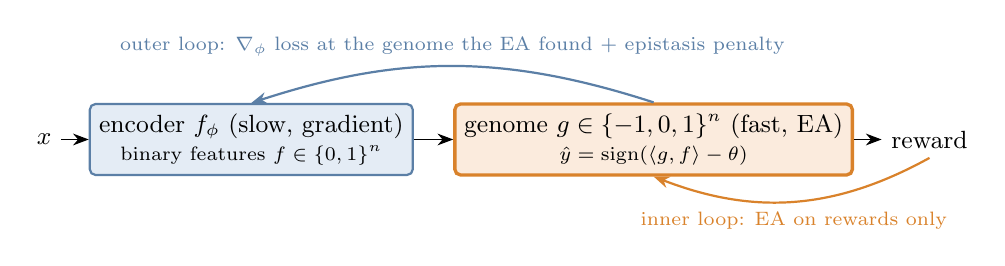
\begin{tikzpicture}[font=\small,>={Stealth[length=2mm]},
 s/.style={draw=slow,fill=slowbg,rounded corners=2pt,thick,align=center,minimum height=0.9cm},
 f/.style={draw=fast,fill=fastbg,rounded corners=2pt,very thick,align=center,minimum height=0.9cm}]
\node (x) {$x$};
\node[s,right=0.35cm of x] (e) {encoder $f_\phi$ (slow, gradient)\\[-1pt]{\scriptsize binary features $f\in\{0,1\}^n$}};
\node[f,right=0.5cm of e] (g) {genome $g\in\{-1,0,1\}^n$ (fast, EA)\\[-1pt]{\scriptsize $\hat y=\mathrm{sign}(\langle g,f\rangle-\theta)$}};
\node[right=0.35cm of g] (r) {reward};
\draw[->] (x)--(e); \draw[->] (e)--(g); \draw[->] (g)--(r);
\draw[->,fast,thick] (r.south) to[bend left=25] node[below,font=\scriptsize]{inner loop: EA on rewards only} (g.south);
\draw[->,slow,thick] (g.north) to[bend right=18] node[above,font=\scriptsize]{outer loop: $\nabla_\phi$ loss at the genome the EA found $+$ epistasis penalty} (e.north);
\end{tikzpicture}
\end{center}

\textbf{Approach and first results on paper.}
\begin{itemize}
\item \textbf{Definition.} The \emph{evolvability} of a representation is the expected number of reward evaluations an EA needs to move between related tasks. It is driven by \emph{epistasis} (ruggedness) and by the \emph{task distance} $k$, the number of genome positions that must change between related tasks.
\item \textbf{Theory.} On additive landscapes, a (1+1)~EA re-adapts from distance $k$ in $O(n\log k)$ evaluations: cost scales with the \emph{size of the change}, not the model. New lemma: for threshold read-outs over binary features,
$|\Delta^2_{ij}F| \le 2\Pr[f_i{=}f_j{=}1,\ |\langle g,f\rangle-\theta|<4]$, so epistasis comes \emph{only} from co-active features near the decision threshold. That is a feature property a training objective can control.
\item \textbf{Method.} \emph{Evolution-in-the-loop} meta-training: an inner EA solves tasks from rewards; the encoder is updated by first-order gradients at the EA's genomes, plus lemma-derived co-activation and margin penalties.
\end{itemize}

\textbf{Plan.}
\begin{itemize}
\item \textbf{Now (CPU cluster, one T4).} (1)~Synthetic task family with known latent factors: measure epistasis, $k$ and evaluations-to-adapt against ground truth. (2)~Images with known factors (dSprites/Shapes3D). (3)~Reward-only adaptation on CIFAR-100 rules.
\item \textbf{Baselines:} multi-task, autoencoder and disentangled encoders; CMA-ES and policy gradients on continuous heads; ES-MAML; a labelled head as reference.
\item \textbf{Go/no-go} after stage~1.
\item \textbf{With compute:} the genome becomes per-expert routing biases in a mixture-of-experts LLM. Evolution-in-the-loop shapes experts and routers so that reward-only domain adaptation is fast. The prompt prefix is shared by the whole population, so $N$ genomes cost roughly one forward pass.
\end{itemize}

\textbf{Novelty.} MAML, ANIL and ES-MAML shape an \emph{initialisation} for a continuous learner. Evolvability ES optimises offspring diversity. LoraHub and C3PO search on top of a \emph{fixed} library. None shapes the representation so that a discrete, reward-only search lands in a landscape class with runtime guarantees. The project connects EA runtime theory, meta-learning and the evolvability literature from biology (Wagner \& Altenberg; Kashtan \& Alon; Clune et al.).

\textbf{Expected output.} A measurable definition of evolvability for learned representations; a feature-level epistasis bound and re-adaptation theory beyond additivity; evolution-in-the-loop training; ground-truth benchmarks; and a scaling path to MoE routing. Full proposal (13~pp.) available on request.
\end{document}
